\documentclass[12pt]{article}

\usepackage{cite}
\usepackage{amstext}
\usepackage{amssymb}
\usepackage{amsmath}
%\usepackage{amssymb}
\usepackage{epsfig}
\usepackage{graphics}
\usepackage{graphicx}

\DeclareMathOperator\erf {erf}


\bibliographystyle{plain}

\begin{document}

\begin{titlepage}

\vfill \LARGE
\begin{center}
Convergence of Analytical Solution
\large

\rule{0mm}{20mm}

O. J.  Halliday, S. D. Griffiths,  D. Parker,

 \vspace{3mm} {\em University of Leeds}


%\rule{40mm}{0.2mm}



\end{center}

\pagestyle{empty}
\end{titlepage}
%
%
%
\section{Limits of Spatial-Temporal Convergence }
\label{sec_background}
%
We aim to study the convergence of our forced forced, lidded system of Parker and Burton, with transient heating function:
%
\begin{equation}
\frac{Q(x,z,t)}{Q_0}= \sin \left( \frac{\pi z }{ H_t} \right) ( H(t) - H(t-T)) ( H(z) - H(z-H_t)) F(x),
\end{equation}
%
where:
%
%
\begin{equation}
F(x) = \sigma_0 \sigma \exp \left( - \frac{x^2}{2 \sigma_0^2 \sigma^2 }\right), \quad 0<z<H_L.
\end{equation}
%
In particular, we wish to find approximate limits (bounds) on the spatial domain and timescales, implicitly imposed by our use of a rigid lid upper boundary condition
on the vertical dimension.  Note that we are interested in the $w$-response only over a smaller range of altitude $z$ such that $0<z< few H_t \ll H_L$. 
%
%
%
\subsection{General Considerations}
%
Considering the above, our sensible heating clearly has a vertical variaton given by the expression:
%
\begin{equation}
\sin\left( \frac{\pi z}{H_t}\right) H(z-H_t).
\end{equation}
%
This heating has a partial Fourier spectrum of:
%
\begin{equation}
\label{equ_partial}
\frac{Q(z)}{Q_0} =  ( H(t) - H(t-T))  \sum_{m=1}^M  b_m \sin \left( \frac{ m \pi }{ H_L} z \right) ,
\end{equation}
%
where:
%
\begin{equation}
 b_m =  \frac{2 \bar{H_t} \pi \sin \left( \bar{H_t} \pi \right) }{ 1 - \bar{H_t}^2 m^2 }, \quad \bar{H_t} = \frac{H_t}{H_L} , \quad M =k H_L,
\end{equation}
%
which is represented in figure \ref{fig_1} below, for a range of $H_L$ values and $H_t = 1$, $\sigma = 1$.  
Note that in general, to ensure convergence, the number of Fourier modes, $M$ used to express the above function scales with lid height $H_L$. 
As the lid is raised, the heating function becomes sharper in relative terms and so it requires more terms in the Fourier series.

To find the location of the peak in the Fourier coefficient set we might try to solve for $m$:
%
\begin{equation}
\frac{db_m}{dm } = 0 \iff \frac{d}{dm} \left(  \frac{\sin \left( \bar{H_t} \pi \right) }{ 1 - \bar{H_t}^2 m^2 } \right) = 0, 
\end{equation}
% 
however this results in a equation for $m$ which requires a numerical solution. Neglecting the numerator and seeking the solution of $1 - m^2 \bar{H}_t^2 = 0$ however, yields:
%
\begin{equation}
m_{max} =  \pm \frac{1}{\bar{H}_t} = \pm \frac{H_L}{H_t} ,
\end{equation}
%
where only the positive root is needed of course. This result is supported by numerical data as follows. Consider the data in figure \ref{fig_1} below. 
Denote the harmonic number of the Fourier series term in equation \ref{equ_partial} with largest $|b_m|$ by $m_{max}$, the range of $m$ over which the 
Fourier coefficients have a significant value by $\Delta m$ and the maximum value of $b_m$ by $b_{max}$. From the data in figure \ref{fig_1} we observe:
%
\begin{equation}
m_{max} \propto \frac{1}{\bar{H}_t} = \frac{H_L}{H_t} , \quad b_{max} \propto \bar{H}_t = \frac{H_t}{H_L}, \quad \Delta m \propto \frac{1}{\bar{H}_t } = \frac{H_L}{H_t}.
\end{equation}
%
%
%
\begin{figure}[h]
\caption{Convergence data. The Fourier series coefficients of in the expanded heating function, for a range of lid heights, for a restricted range of $m_z$ (upper) and $k_z = \frac{2m}{H_L}$ (middle).
 As the lid height is raised the distribution of Fourier coefficients (i) centres on larger $m$, (ii) broadens and (iii) has a peak value which reduces. This behaviour clearly underscores the need to increase the upper limit of $m$ in summation equation \ref{equ_partial}. These trends are clearly confrimed in the lower panel which shows the value of $H_L b_m$  as a function of $k_z$- clearly all data in the
top panels has collapsed onto a single set of coefficients.  } 
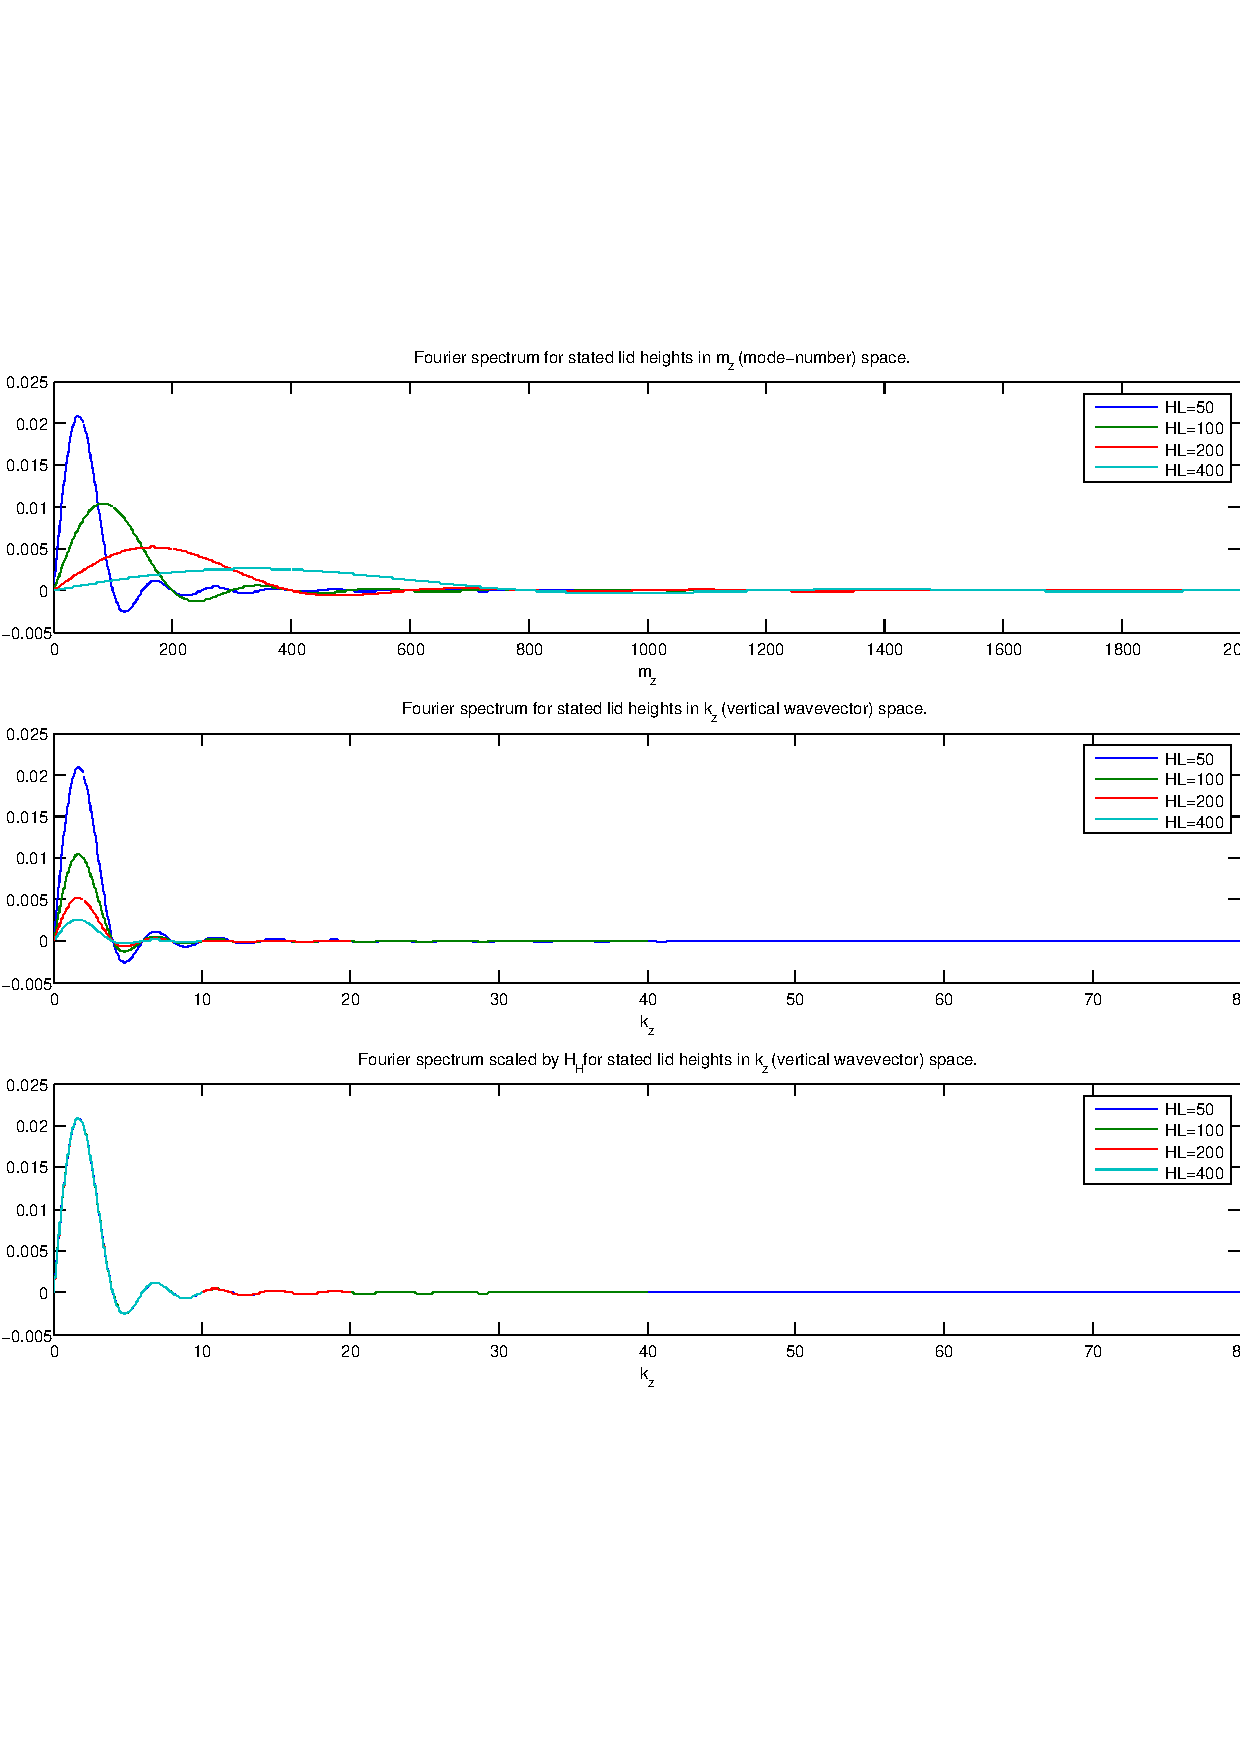
\includegraphics[scale=0.8,angle=0] {fig1.pdf} 
\label{fig_1}
\end{figure}
%
%
%
Now, the significant terms in the Fourier series have a value which is, broadly, proportional to $\bar{H}_t$. The number of significant terms is, broadly, proportional to $\frac{1}{\bar{H}_t}$ then 
for the summation in equation \ref{equ_partial}
%
\begin{equation}
\sum_{m=1}^M  b_m \sin \left( \frac{ m \pi }{ H_L} z \right) \approx \bar{H}_t \times \frac{1}{\bar{H}_t} = constant,
\end{equation}
%
which suggests a similar scale of response whatever the lid-height.

From figure \ref{fig_1}, the mode numbers $m$ which contribute most significantly to the computed $w$-response increase as the lid height increases. 
(These most significant modes correspond to the peak in the Fourier spectrum, note). They will give similar contributions over the visualization region as lid-height increases.
We can see this as follows.  For $s=0$ the $w$-response is written as a sum of contrinbutions (modes) moving with horizontal speed $c(m)$:
%
\begin{equation}
\label{equ_response}
\frac{w}{Q_0} = \frac{1}{N^2} \sum_{m-1}^M b_m \sin \left( \frac{m \pi}{H_L} z\right) F(x - c t), \quad c(m) = \frac{N H_L}{ m \pi}.
\end{equation}
%
As we have seen, for the largest and most significant Fourier coefficients $m \approx \frac{H_L}{H_t}$, hence by substituting this value, 
we can approximate the spatial variation of the significant terms in the above $w$-response:
%
\begin{equation}
\sin \left( \frac{m \pi}{H_L} z\right) F(x - c t) \approx \sin \left( \frac{H_L \pi}{H_t H_L} z\right) F \left( x - \frac{N H_L H_t}{ H_L \pi} t \right),
\end{equation}
%
and cancelling factors of $H_L$, all significant modes are seen (i) to have similar vertical variation within the heating region $0<z<H_t$ and (ii) to
move at a speed which is independent of the lid-height and determined by the height of heating, $H_t$: 
%
\begin{equation}
\sin \left( \frac{m \pi}{H_L} z\right) F(x - c t) \approx \sin \left( \frac{\pi}{H_t} z\right) F \left( x - \frac{N H_t}{ \pi} t \right),
\end{equation}
%
We return to this point later.

In conclusion, the variation of the $w$-response over the heating region is likely to be qualitatively similar when as lid height is varied. 
i.e. the $w$-response will look qualitatively similar and have a similar range. So, for example, the lid height $H_L$ will not strongly affect the characteristic scale of the response 
however it must be expected to change details. The change in these details will be small when a sufficient lid-height has been used. This is clear in figure \ref{fig_1a} below 
where the $w$-response for $H_L=100H_t$ and $H_l=3H_t$ are shown and compared. Both responses lie within the approximate range $-2000<\frac{w}{Q_0}<6000$ and are 
qualitatively similar but their difference (bottom part of figure), whilst an order of magnitude smaller ($-200<\frac{\Delta w}{Q_0}<400$) is still significant. Note that the two responses
cancel at the location of the heating.
%
%
%
\begin{figure}[h]
\caption{Comparison of two $w$-responses for $t=1000s$ for lid height $H_L=200H_t$ (top) and $H_L=30H_t$ (middle) and their difference (bottom). The region
over which these fields are compared only occupies to $0<z<3H_t$ note- the difference is not defined outside this range of $z$.} 
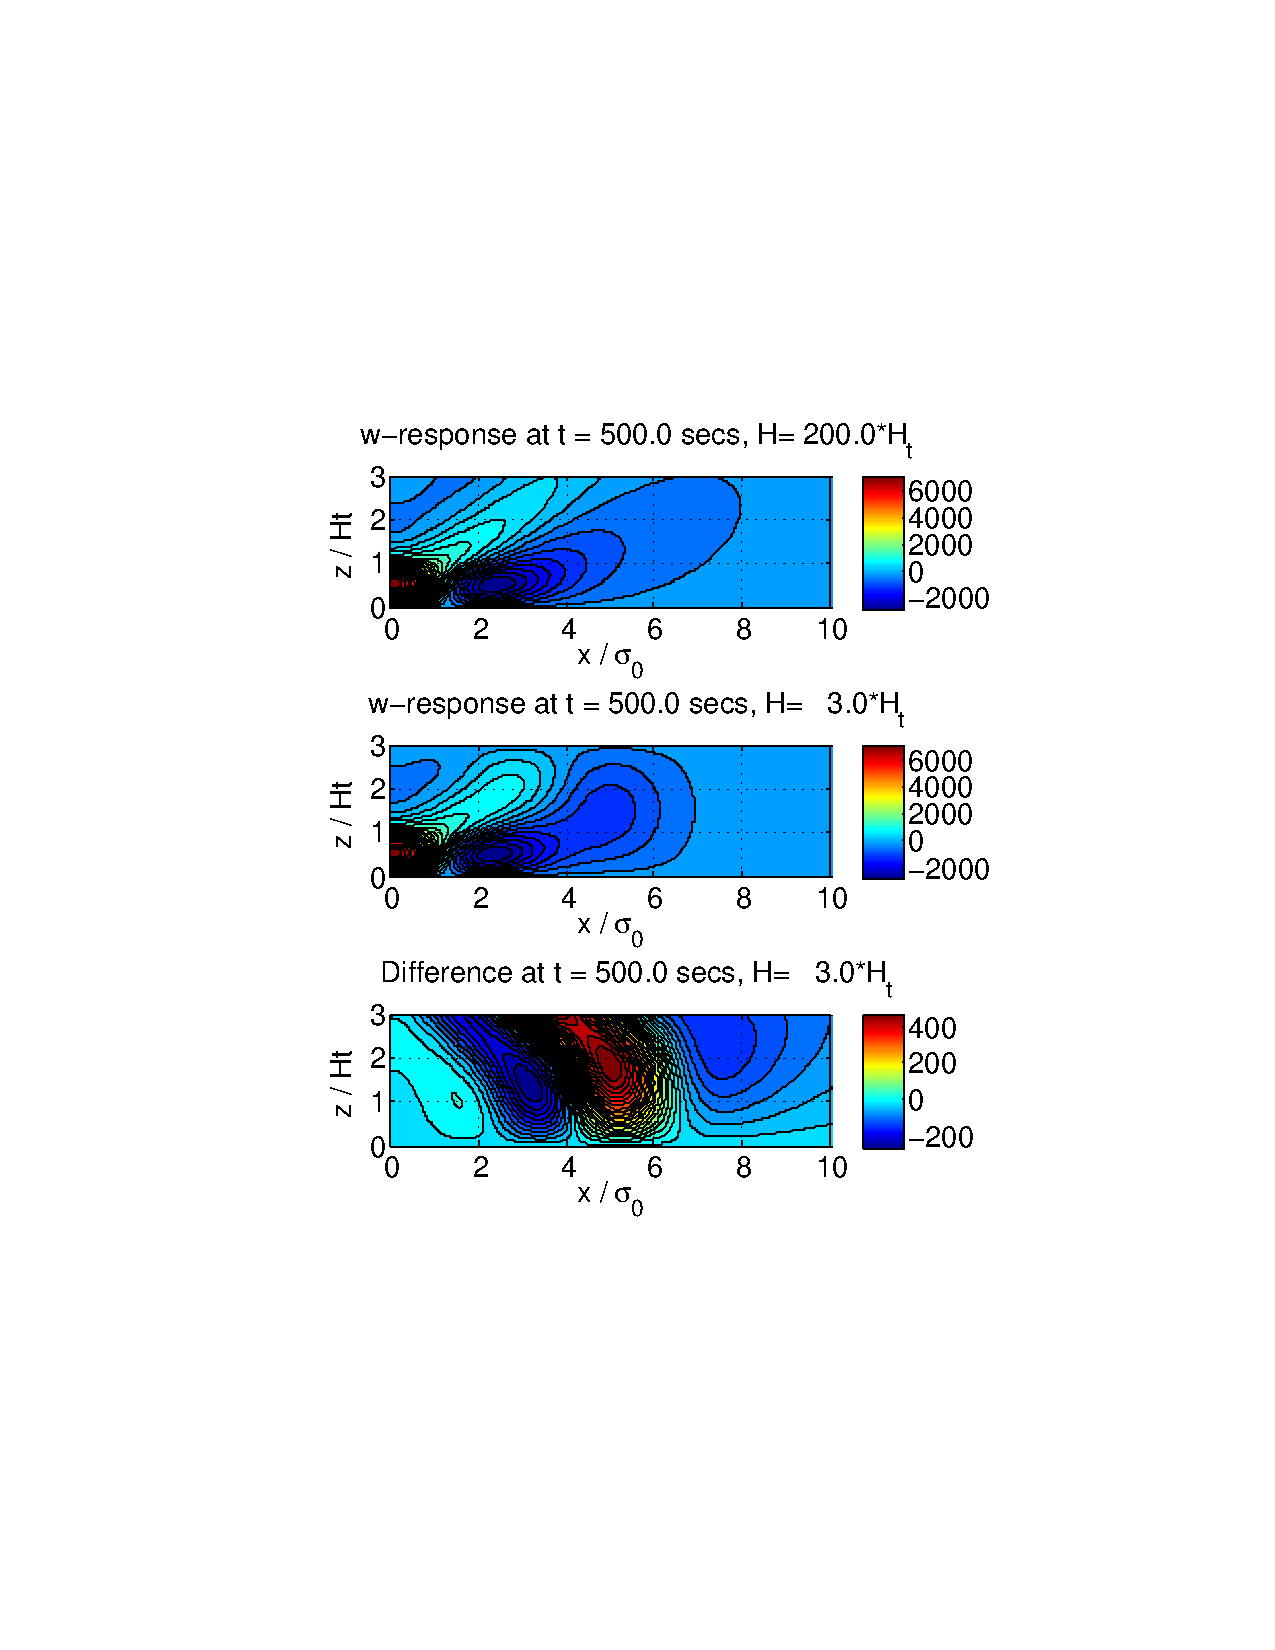
\includegraphics[scale=0.8,angle=0] {fig1a.pdf} 
\label{fig_1a}
\end{figure}
%
%
%
\subsection{Quantifying the Influence of $H_L$ and $\sigma$}
%
Broadly, the $w$-response is comprised of bores of $w$ perturbation which extend approximately radially, from the fixed source of heat to the right and left (left not shown in figure)
as they elongate radially, weaken and descend. This response is apparent in the shapshot of the logarithm of the $w$-response in figure \ref{fig_2} below. 
%
%
%
\begin{figure}[h]
\caption{The $w$-response. Left panel is $\log_e(|w|)$, right panel $w$. The radial bores are visible in the plot on the left: the principal contribution is more clear on the light. 
The subset of $b_m$, $m<200$ are mainly responsible for each the features in the panel on the right. } 
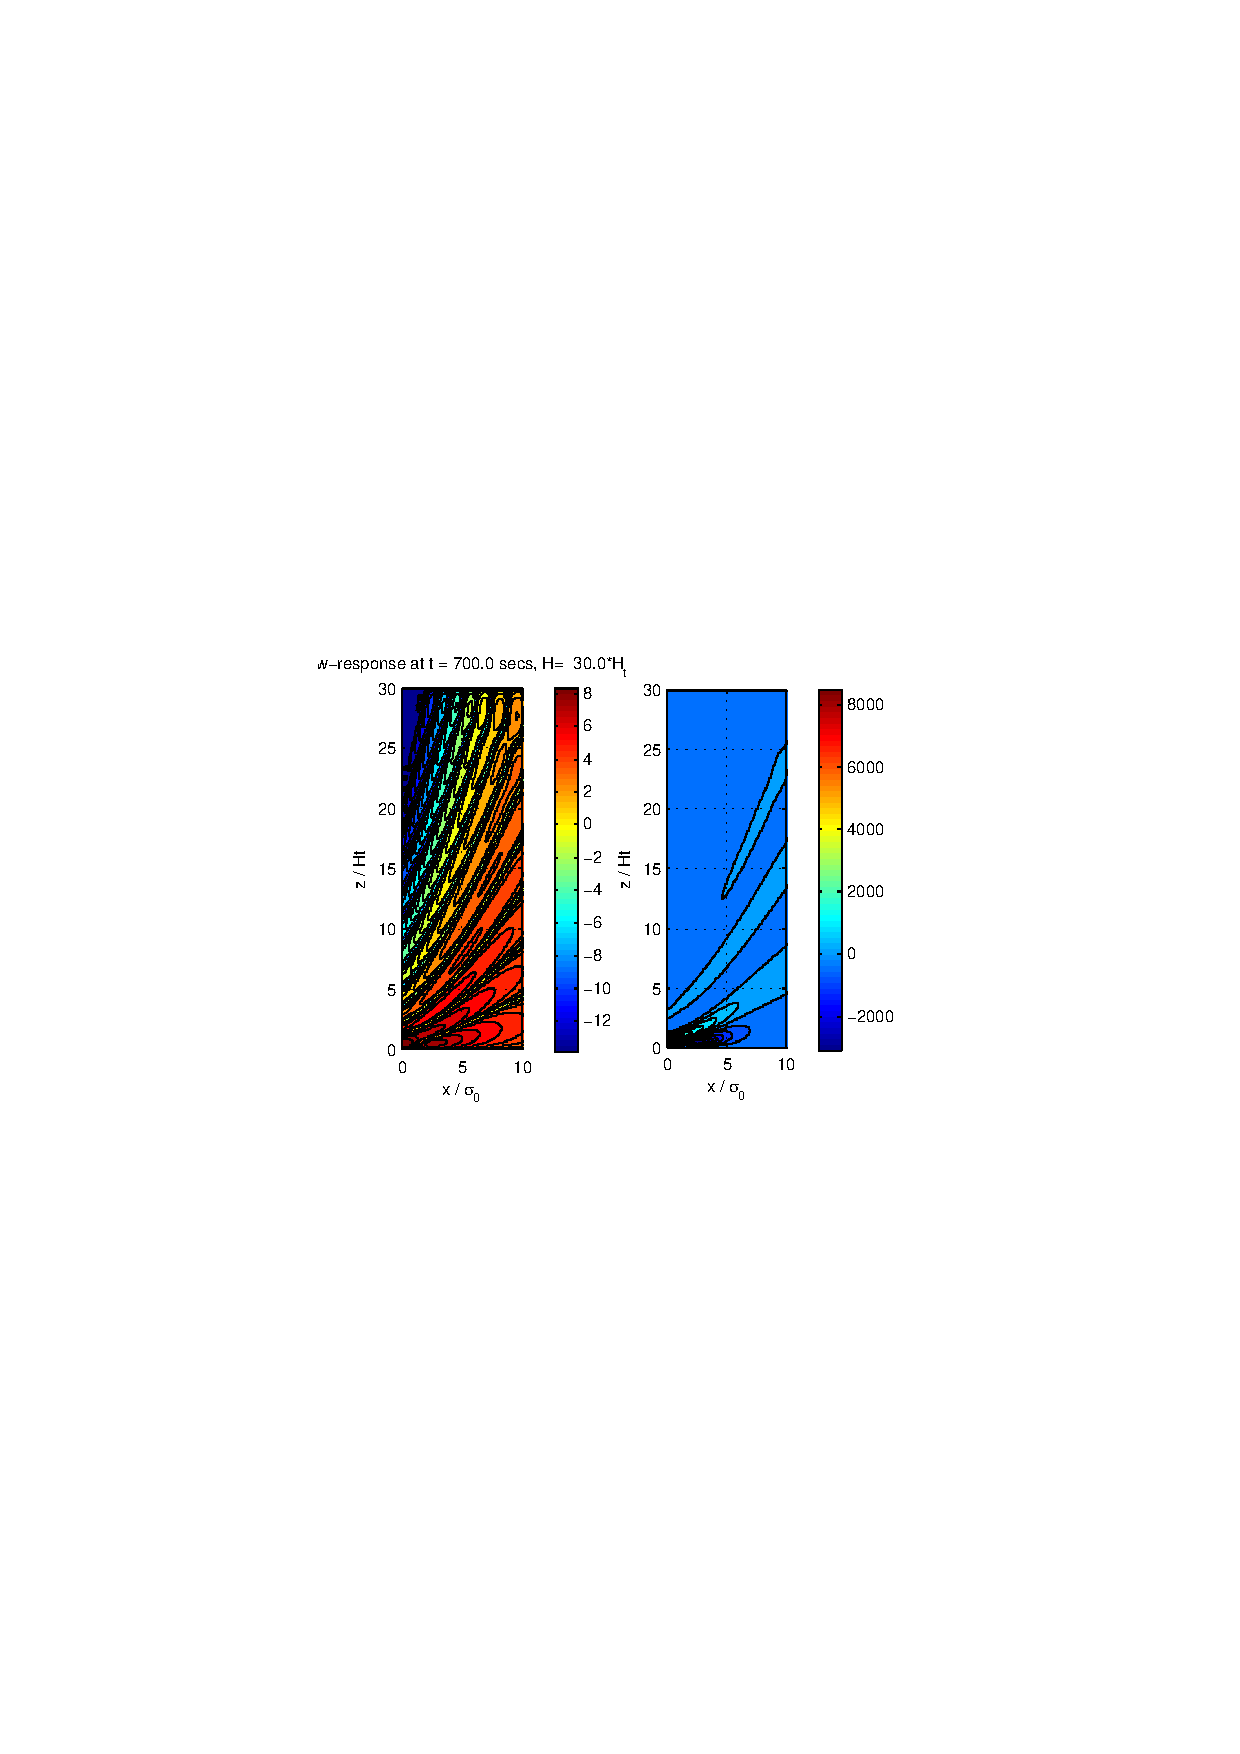
\includegraphics[scale=1.0,angle=-0] {fig2.pdf} 
\label{fig_2}
\end{figure}
%
%
%

Model the forced response on freely propagating gravity waves in an un-lidded slab, described by the Boussinesq approximation.
This is more valid than it might seem when you consider how the $w$-response 
in equation \ref{equ_response} is made-up of propagating contributions like $\frac{b_m}{N^2} \sin \left( \frac{m \pi}{H_L} z \right) F(x - c t)$. 
The free gravity waves in such a system are characterised by a vertical wavelength (wavenumber) $\lambda_z$ ( $k_z$ ).
For our data, we estimate this wavelength from the most significant Fourier series terms (with largest $b_m \approx b_{max} $), which have vertical wavelengths:
%
\begin{equation}
\label{equ_1}
\lambda_z \approx \frac{H_L}{m_{max} } \iff k_z = \frac{2 \pi }{\lambda_z} = \frac{ 2 m_{max} \pi }{ H_L }.
\end{equation}
%
Recall $m_{max} = \frac{H_L}{H_t}$ hence:
%
\begin{equation}
k_z =  \frac{ 2H_L \pi }{ H_t H_L } = \frac{2 \pi }{ H_t}, \quad \quad \forall H_L
\end{equation}
%
The horizontal wavelength and wavevector must also be estimated. We take the full width at half maximum ( $\sigma$ ) of the function 
which describes the horizontal variation of heating, $F(x)$:
%
\begin{equation}
\label{equ_2}
\lambda_x = \sigma \sigma_0 \iff k_x = \frac{2 \pi}{ \lambda_x} = \frac{2 \pi }{\sigma \sigma_0}.
\end{equation}
%
Therefore the group and phase velocities of our "heat-induced gravity waves" is, by assumption, given by [GAFD equ 2.32]:
%
\begin{equation}
\underline{c_g} = \pm \frac{N k_z}{( k_x^2 + k_z^2)^{3/2}} ( k_z,0,-k_x), \quad \underline{c_p} =   \frac{N }{k_x^2 + k_z^2} ( k_x,0,k_z),
\end{equation}
%
where the it is understood that the above expression for group speed 
will be evaluated at those value of $k_x$ and $k_z$ which characterise the wavepacket in question.
Hence, we evaluate $\underline{c_g}$ using equations \ref{equ_1} and \ref{equ_2}:
%
\begin{equation}
\label{equ_cg}
\underline{c_g} = \pm \left( \frac{ \sigma \sigma_0 N }{\pi} \right)  \frac{ R^2 }{(1 + R^2 )^{3/2}} \left( 1,0,-\frac{1}{R }\right),
\end{equation}
%
where we have defined the dimensionless ratio parameter
%
\begin{equation}
R = \frac{\sigma \sigma_0}{ H_t} 
\end{equation}
%

As $R$ increases (decreases) corresponding to less (more) localised heating, the vertical component of the group velocity will decrease (increase). 
The group velocity vector is tilted downwards as the heating becomes more localised i.e. as $\sigma$ decreases.
More formally, we may assess the rotation of the group velocity vector as the width of the applied heating is varied. 
The angle subtended at the horizontal by $\underline{c_g} $ is:
%
\begin{equation}
\alpha \equiv \angle \underline{c_g} = \tan^{-1} \left( \frac{-\frac{1}{R} }{ 1 } \right) = \tan^{-1} \left( - \frac{1}{R } \right) =  \tan^{-1} \left( - \frac{H_t}{ \sigma \sigma_0 } \right).
\end{equation}
%
Here a negative angle indicates a downward direction. Note the above is correct for both $\pm$ cases in equation \ref{equ_cg}. Clearly, 
the modulus of angle $\alpha$ increases as the width of the heating function decreases (i.e. $\sigma \sigma_0$ decreases). This means that 
$\underline{c_g} $ may be said to rotate towards the vertical as the width of heating decreases i.e. the heating function becomes "sharper".
For completeness, the group speed is given by taking the modulus in equation \ref{equ_cg}:
%
\begin{equation}
\label{equ_cg}
c_g = |\underline{c_g}| = \left( \frac{ \sigma \sigma_0 N }{\pi} \right)  \frac{ R}{(1 + R^2 ) }.
\end{equation}
%
Remark. Is it worth considering how this varies with heating width?
 
To assess the influence of the lid on our calculations let us estimate the time, $\Delta t $ taken for an "error" in the $w$-response caused by the lid i.e. located at $z=H_L$ to traverse the slab:
%
\begin{equation}
\label{equ_dt}
\Delta t = \frac{H_L}{c_{gz}} = \frac{ H_L \pi (1 + R^2 )^{3/2} } {\sigma \sigma_0 N R }. 
\end{equation}
%
For deep convection, which spans the troposphere we take the ratio of horizontal and vertical storm scales to be small:
%
\begin{equation}
\frac{\sigma \sigma_0}{ H_t} \approx \frac{1}{10},
\end{equation}
%
therefore we can neglect $R^2$ in the numerator:
%
\begin{equation}
\Delta t \approx \frac{H_L \pi}{ \sigma \sigma_0 N R },
\end{equation}
%
and substituting for $R$ we have the estimate:
%
\begin{equation}
\Delta t  = \frac{\pi}{N} \frac{H_L H_t}{ \sigma^2 \sigma^2_0} =  \frac{\pi}{N} \frac{H_t^2}{ \sigma^2 \sigma^2_0} \frac{H_L}{H_t} = \frac{\pi}{N} \frac{1}{R^2} \frac{H_L}{H_t},
\end{equation}
%
which increases with lid height, as expected,  note. Therefore, for a moderate lid height $H_L = 10 H_t$ we estimate:
%
\begin{equation}
\Delta t > \frac{\pi}{N} \frac{1}{R^2} \frac{H_L}{H_t} = 3 \times 10^2 \times 10^2 \times 10 = 3 \times 10^5 s.
\end{equation}
%

Consider the influence on the horizontal scales. Still using our gravity wave model, the lid will affect positions:
%
\begin{eqnarray}
\Delta x & = & c_{gx} \Delta t =  \frac{ \sigma \sigma_0 N R^2}{ \pi (1 + R^2)^{-3/2}}  \frac {H_L \pi (1+R^2)^{3/2}} { \sigma \sigma_0 N R } , \\ \nonumber
            & = & H_L R, \\ \nonumber
\end{eqnarray}
%
where we have used equations \ref{equ_cg} and \ref{equ_dt}.  Hence, in conclusion, since both $\Delta t$ and $\Delta x$ are proportional to $H_L$, it should be possible to choose a lid height to allow us to study a region and time-frame free from the effects of the lid.
%
\begin{equation}
\Delta x \approx \frac{H_L}{30}, \quad \quad \Delta t \approx 3 \times 10^5 H_L s.  \\ \nonumber
\end{equation}
%
%
%
\subsection{Relating time-scale and Box Length}
%
Recall, all contributions to the $w$-response of the Parker and Burton system are of the form 
$\frac{b_{m_z}}{N^2} \sin \left( \frac{m \pi}{H_l} z \right) \exp \left( - \frac{(x \pm \frac{NH_L}{m \pi} )}{x} \right)$. This 
structure or mode propagates left or right (not considered) at speed:
% 
\begin{equation}
\frac{dx}{dt} = \frac{NH_L}{\pi m},
\end{equation}
%
and it will be centred on location:
% 
\begin{equation}
x = \frac{NH_L t}{\pi m}, 
\end{equation}
%
which may or may not lie in the domain- only higher-order modes (larger $m_z$) stay inside the box $0<x<x_{max}$ at given $t$. Note, the larger $H_L$, the faster all modes leave the domain. For the box, or visualisation region to contain the principal modes ($m \approx m_{max}=\frac{H_L}{H_t}$) the above becomes:
% 
\begin{equation}
x = \frac{NH_L  H_t t}{\pi H_L} = \frac{N H_t t}{\pi}. 
\end{equation}
%
Hence, if we want all the important contributions to the Fourier-series expanded $w$-response to be in our calculations we must make certain 
that the box length, $\Delta x$, and chosen time since the start of heating, $\Delta t$, are related such that:
 % 
\begin{equation}
\Delta x >  \frac{N H_t }{\pi} \Delta t. 
\end{equation}
%

This is important- modes which have left the domain clearly won't contribute to our convergence calculations. 
Hence it is possible that convergence with lid hight might be dominated by different modes at different times. 
For example, for $H_L = 3 H_t$ (small) the mode with the largest amplitude $b_{m_z}$ has a relatively small $m_{max}= 26$ 
and at $t=1000s$ it will have reached distance:
% 
\begin{equation}
x = \frac{0.01 \times 3 \times 1000 }{ 26 \pi } \approx 0.3,
\end{equation}
%
which must lie inside the box if our results are to be sensible, so $\Delta x > 0.3$ is needed.

In fact, given the Fourier-series cut-off, $M$, we can count the number of modes, $N_0$, which are inside the domain at time $t$:
%
\begin{equation}
N_0 = M - \frac{NH_L \Delta t }{\pi \Delta x} = kH_L -   \frac{NH_L \Delta t }{\pi \Delta x} = H_L \left( k - \frac{N \Delta t }{\pi \Delta x} \right).
\end{equation}
%
Here, we have used the fact that modes with $m$: $\Delta x > \frac{N H_L \Delta t}{ \pi m}$ will be inside the box (i.e. modes with
$m>\frac{NH_L \Delta t }{\pi \Delta x}$ will be counted) and the partial Fourier-series cut-off is given by $M = k H_L$.

Clearly it is not correct to assume convergence will be similar at all times: at very short times $w$-response fields may be 
dominated by the modes with the largest Fourier coefficients whereas for larger time 
it may the only modes which lie in the domain may have large $m_z$. The data support this observation: see below.
%
%
%
\section{Discussion}
%
To observe convergence (or not!) of our data with lid height we consider domain:
%
\begin{equation}
0<\frac{x}{\sigma_0}<10, \quad 0<\frac{z}{H_t}<2,
\end{equation}
% 
with a lid height of $H_L = 1024H_t$ defining the infinite or converged system. Let us define difference field:
%
\begin{equation}
\Delta w (x,z,t,H_L) = w(x,z,t,H_L,\sigma) - w(x,z,t,1024H_t,\sigma).
\end{equation}
%
We consider the variation with $H_L$ of (i) the rms value of the absolute difference field (or 2D Matlab array (x-y mesh)):
%
\begin{equation}
\Delta w_{rms} (x,z,t,H_L) = \sqrt{  \frac{ \sum_{x} \sum_{z} \left(  w(x,z,t,H_L,\sigma) - w(x,z,t,1024H_t,\sigma)  \right)^2 } { N_x N_z} }, 
\end{equation}
%
or (ii) the maximum of the absolute difference field:
%
\begin{equation}
 max \left(  \sqrt{ \left( w(x,z,t,H_L,\sigma) - w(x,z,t,1024H_t)  \right)^2 } \right).
\end{equation}
%
or (iii) the  rms value  of the \emph{ relative } difference field:
%
\begin{equation}
 \sqrt{  \frac{ \sum_{x} \sum_{z} \left(  \frac{w(x,z,t,H_L,\sigma) - w(x,z,t,1024H_t,\sigma)}{w(x,z,t,1024H_t,\sigma)} \right)^2 } { N_x N_z} },
\end{equation}
%
or (iv) the maximum of the \emph{ relative } difference field:
%
\begin{equation}
max \left(  \sqrt{ \left(  \frac{ w(x,z,t,H_L,\sigma) - w(x,z,t,1024H_t) }{ w(x,z,t,1024H_t) } \right)^2 } \right),
\end{equation}
%
or (v) Doug's quantity:
%
\begin{equation}
 \frac{ \Delta w_{rms} (x,z,t,H_L) } { w_{0 rms} }, \quad w_{0 rms} = \sqrt{  \frac{ \sum_{x} \sum_{z} \left(  w(x,z,t,1024H_t,\sigma)  \right)^2 } { N_x N_z} }
\end{equation}
or (vi) Doug's second quantity:
%
\begin{equation}
 \frac{ \Delta w_{rms} (x,z,t,H_L) } {max ( w_0 ) }, \quad max( w_0 ) =max \sqrt{   \left(  w(x,z,t,1024H_t,\sigma)  \right)^2  }
\end{equation}
% 
We present below linked scatter plots of quantities (i)....(vi) defined above with heating width $\sigma$ as a the parameter of the set of curves produced.  In the data in figure \ref{fig_conv1} for a range of $\sigma$ and $2<H_L<1024$ we see non-uniform convergence which is more rapid for larger $\sigma$ (or FWHM) i.e. smoother horizontal variation of horizontal heating. The same trends with $\sigma$ are there for shorter time $t=200$ in figure \ref{fig_conv4} but now the convergence is more uniform and slower. Note that the difference-field data have much smaller values when Doug's definition is used. 
%
%
%
\begin{figure}[h]
\caption{Linked scatter plots of convergence of the $w$-response vs. lid height, $H_L$ at time $t=1000s$.
Left (right) two panels show absolute convergence data such as $log_{10}(\Delta w_{rms})$ vs. $log_{10}(H_L)$, the middle two panels 
show correponding relative data and the right two panels show alternative relative data. The value of $\sigma$ increases downwards in each plot, note.
Note also that the convergence data obtained using Doug's definition shows a similar trend to the others however the
values recorded are smaller by about three orders of magnitude. We make further remarks below. 
The raw data on which this summary is based is shown in figures \ref{fig_conv2} and \ref{fig_conv3}. } 
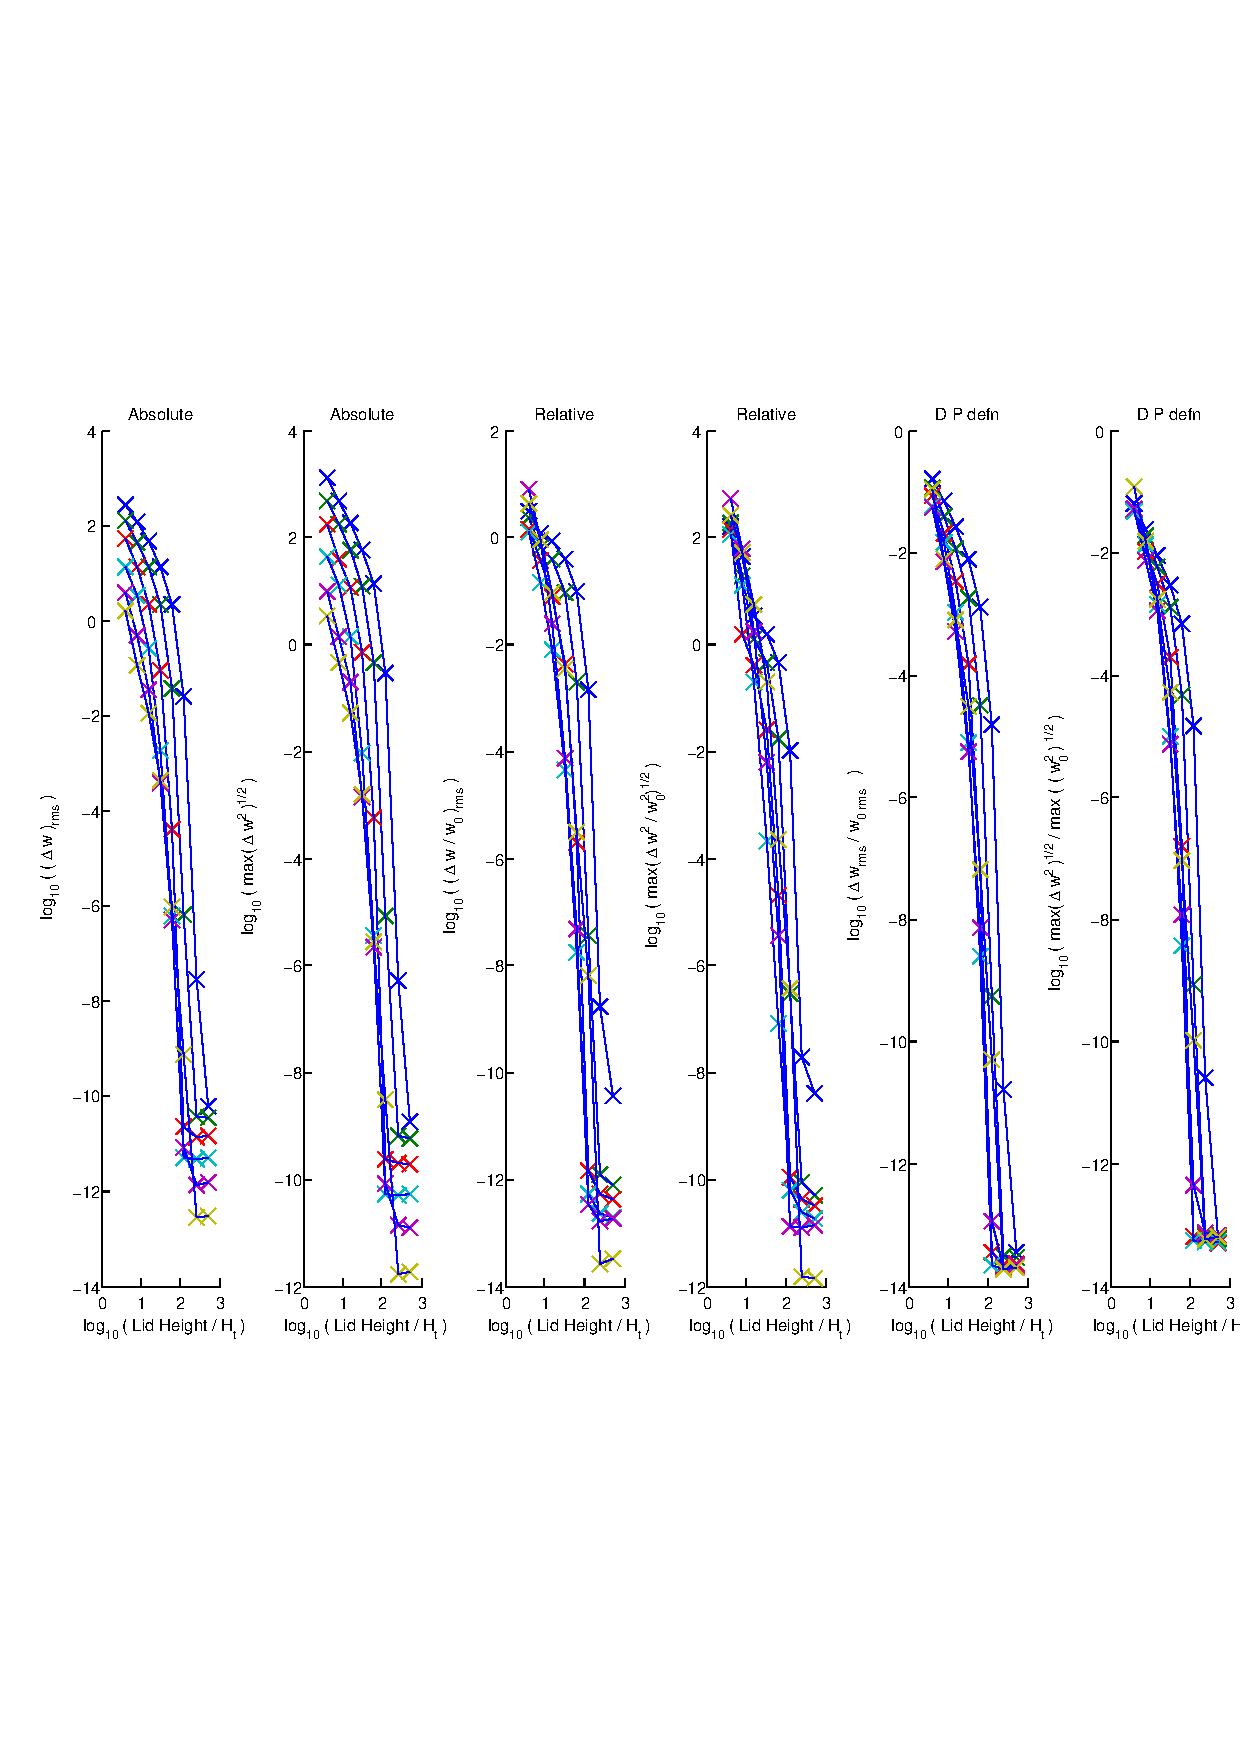
\includegraphics[scale=0.8,angle=-0] {fig4a.pdf} 
\label{fig_conv1}
\end{figure}
%
%
%
\begin{figure}[h]
\caption{The raw data on which summary convergence plot \ref{fig_conv1}. This data has $\sigma=FWHM = 1$ (narrow horizontal heating). } 
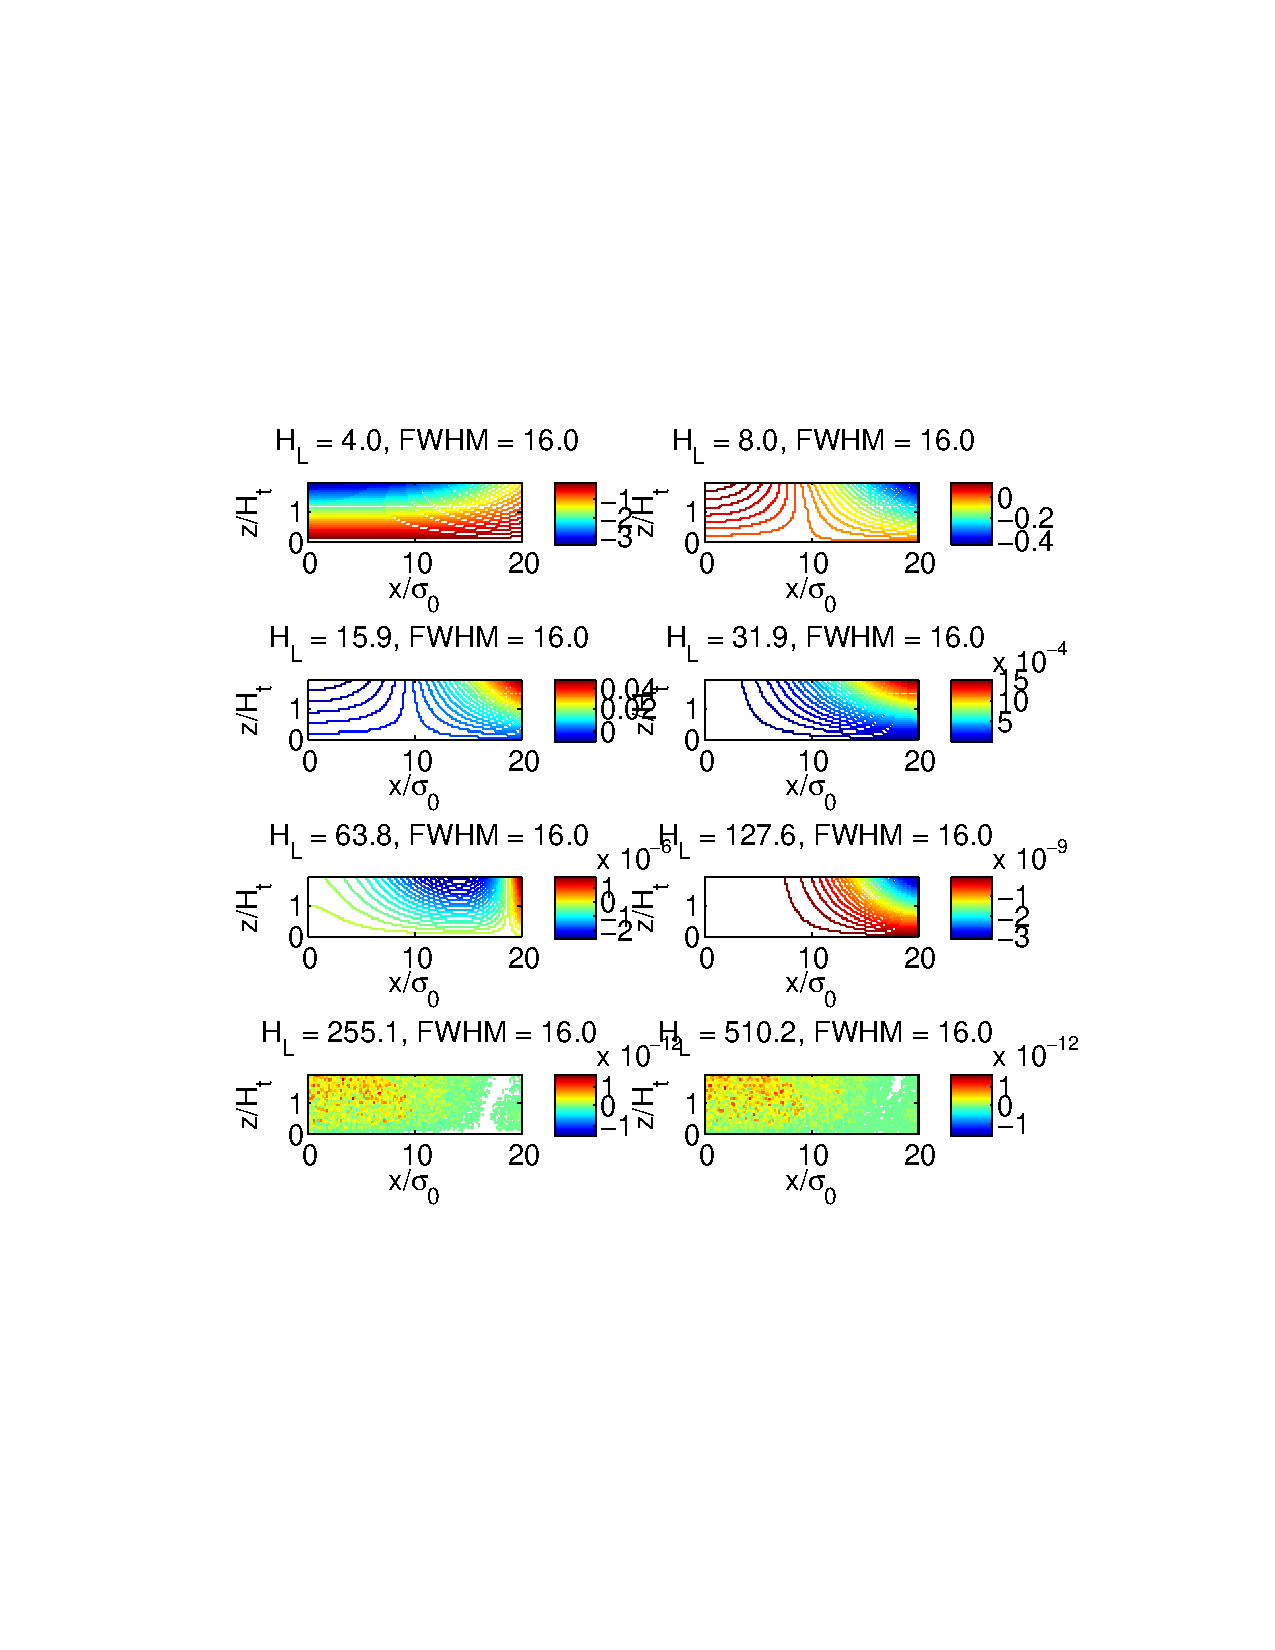
\includegraphics[scale=0.8,angle=-0] {fig4c.pdf} 
\label{fig_conv2}
\end{figure}
%
%
%
\begin{figure}[h]
\caption{The raw data on which summary convergence plot \ref{fig_conv1} is based. This data has $\sigma=FWHM=16$ (broad horizontal heating function) } 
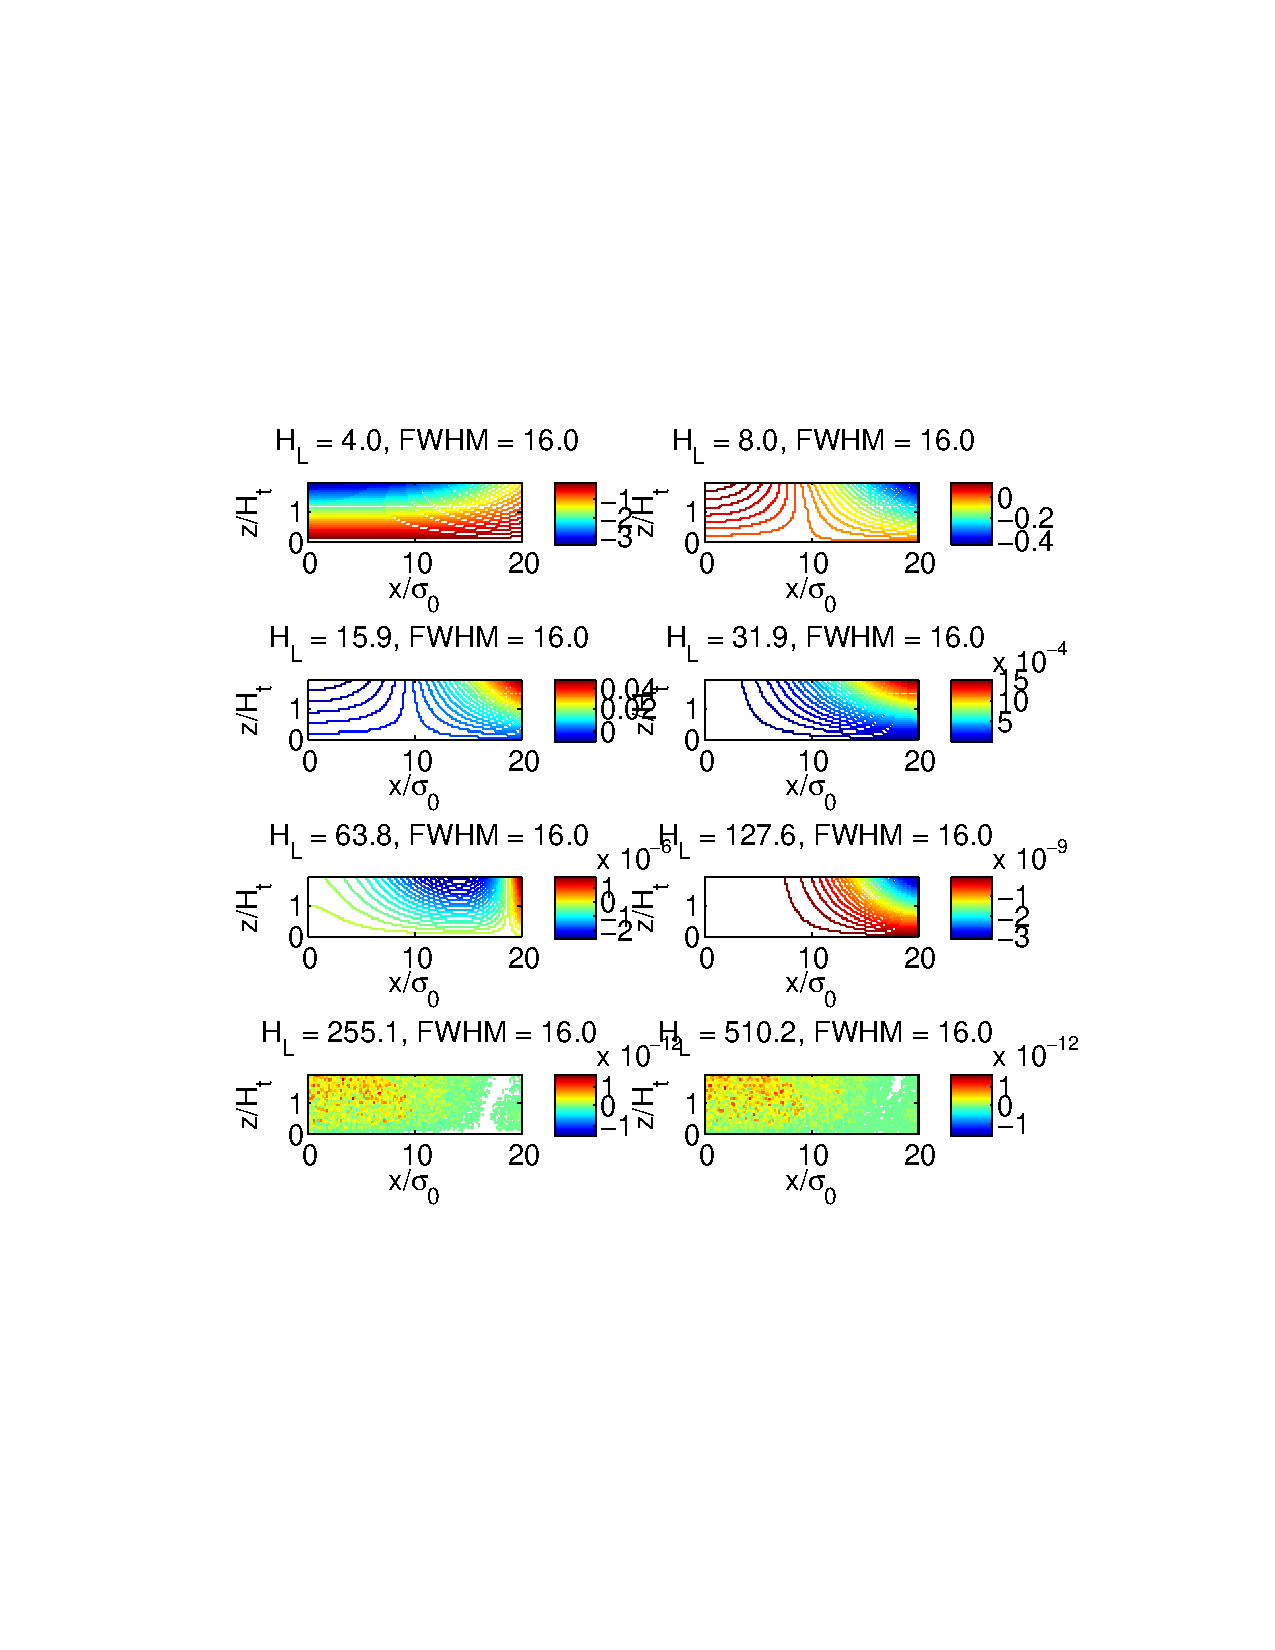
\includegraphics[scale=0.8,angle=-0] {fig4c.pdf} 
\label{fig_conv3}
\end{figure}
%
%
%
%
%
%
\begin{figure}[h]
\caption{Linked scatter plots of convergence of the $w$-response vs. lid height, $H_L$ at smaller time $t=200s$.
Note the qualitative differences between this plot and the corresponding plot at $t=2000s$. } 
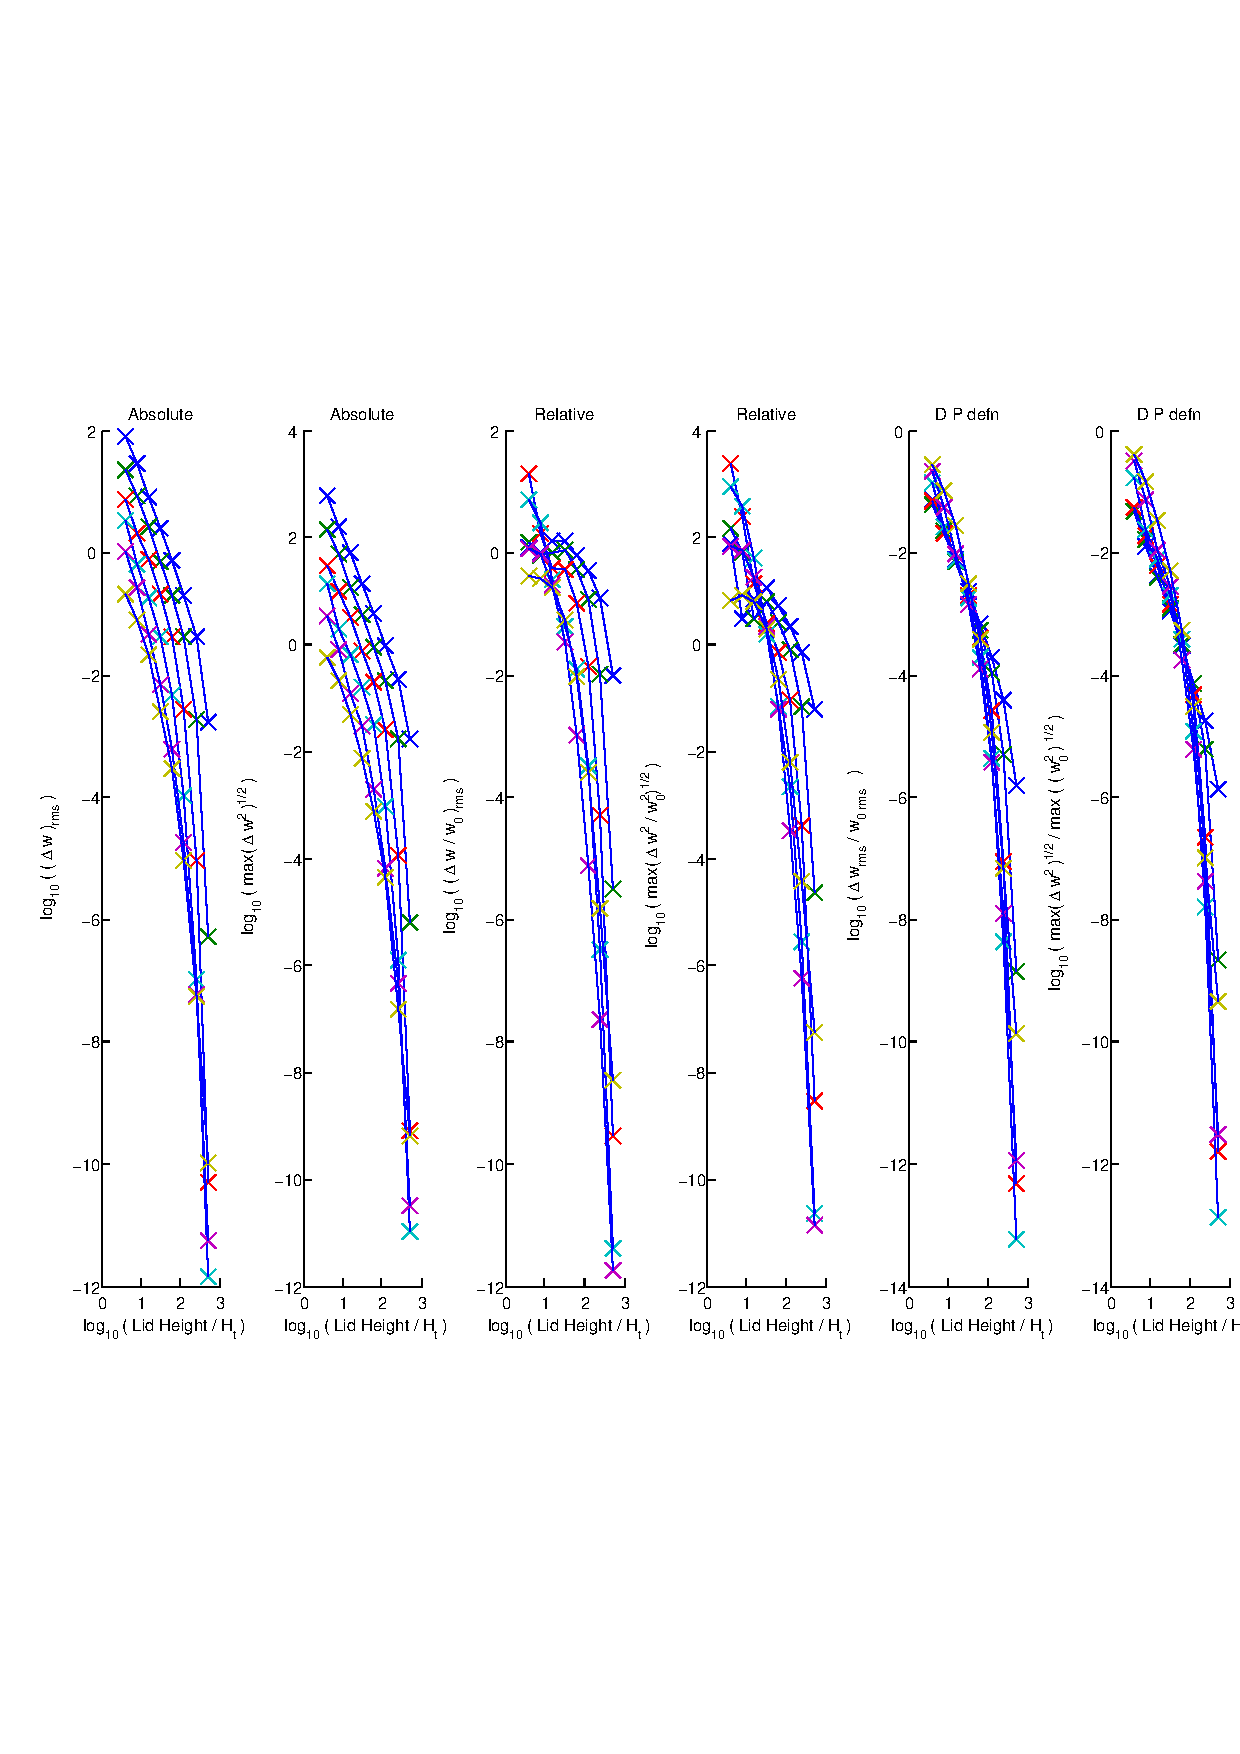
\includegraphics[scale=0.8,angle=-0] {fig4d.pdf} 
\label{fig_conv4}
\end{figure}

{ \bf Remarks }

(i) trends are pretty universal: the convergence graphs all look qualitatively the same across all the methods of measuring convergence we have used. 

(ii) Convergence is generally not uniform with lid height. In plots of e.g. $\Delta w_{rms} (t,H_L,\sigma)$ vs. $log_{10} (H_L)$ over the range of $\sigma$ in figure \ref{fig_conv1}
the negative (good!) gradient increases in modulus (convergence speeds-up?) as $H_L$ increases, again over the range of $\sigma$. Generally slow convergence is followed by faster convergence (the modulus of the gradient increases).

(iii) Convergence plots obtained at different $t$ values differ. 

(iv) Convergence is generally faster (higher-order?) with larger $\sigma$. Recall, total heating is conserved but larger $\sigma$ means heating input is horizontally spread, with a more gentle horizontal variation. This observation may be explained as follows. For all $H_L$, adding, or superposing smoother functions (with larger $\sigma$) must give a smoother result, which means that large differences between $w(x,z,t,H_L,\sigma)$ and $w(x,z,t,1024H_t, \sigma)$ will be smoothed 
so $\Delta w_{max} (H_L,\sigma)$ will must be reduced and the convergence will therefore improve generally as $\sigma$ increases

(v) Using Doug's definition of a relative difference field causes the data for convergence at different $\sigma$ to "collapse" onto one curve. This is particularly noticeable at
the shorter time considered in figure \ref{fig_conv4} though the effect is still there in figure \ref{fig_conv1}. 





























\end{document}